% !TEX TS-program = xelatex
% !BIB program = bibtex
% !TeX spellcheck = ru_RU

% About magic macroses see also  
% https://tex.stackexchange.com/questions/78101/ 

% Этот шаблон ВКР: https://github.com/spbu-se/matmex-diploma-template
% Ревизия на момент написания ВКР: 1c0b998 (May 16, 2022)

% По умолчанию используется шрифт 14 размера. Если нужен 12-й шрифт, уберите опцию [14pt]
\documentclass[14pt
  , russian
  %, xcolor={svgnames}
  ]{matmex-diploma-custom}
\usepackage[table]{xcolor}
\usepackage{graphicx}
\usepackage{tabularx}
\newcolumntype{Y}{>{\centering\arraybackslash}X}
\usepackage{amsmath}
\usepackage{amsthm}
\usepackage{amsfonts}
\usepackage{amssymb}
\usepackage{mathtools}
\usepackage{thmtools}
\usepackage{thm-restate}
\usepackage{tikz}
\usepackage{wrapfig}
% \usepackage[kpsewhich,newfloat]{minted}
% \usemintedstyle{vs}
\usepackage[inline]{enumitem}
\usepackage{subcaption}
\usepackage{caption}
%\usepackage[nocompress]{cite}
\usepackage{makecell}
% \setitemize{noitemsep,topsep=0pt,parsep=0pt,partopsep=0pt}
% \setenumerate{noitemsep,topsep=0pt,parsep=0pt,partopsep=0pt}


\graphicspath{ {resources/} }

% 
% % \documentclass 
% %   [ a4paper        % (Predefined, but who knows...)
% %   , draft,         % Show bad things.
% %   , 12pt           % Font size.
% %   , pagesize,      % Writes the paper size at special areas in DVI or
% %                    % PDF file. Recommended for use.
% %   , parskip=half   % Paragraphs: noindent + gap.
% %   , numbers=enddot % Pointed numbers.
% %   , BCOR=5mm       % Binding size correction.
% %   , submission
% %   , copyright
% %   , creativecommons 
% %   ]{eptcs}
% % \providecommand{\event}{ML 2018}  % Name of the event you are submitting to
% % \usepackage{breakurl}             % Not needed if you use pdflatex only.
% 
% \usepackage{underscore}           % Only needed if you use pdflatex.
% 
% \usepackage{booktabs}
% \usepackage{amssymb}
% \usepackage{amsmath}
% \usepackage{mathrsfs}
% \usepackage{mathtools}
% \usepackage{multirow}
% \usepackage{indentfirst}
% \usepackage{verbatim}
% \usepackage{amsmath, amssymb}
% \usepackage{graphicx}
% \usepackage{xcolor}
% \usepackage{url}
% \usepackage{stmaryrd}
% \usepackage{xspace}
% \usepackage{comment}
% \usepackage{wrapfig}
% \usepackage[caption=false]{subfig}
% \usepackage{placeins}
% \usepackage{tabularx}
% \usepackage{ragged2e}
% \usepackage{soul}
\usepackage{csquotes}
% \usepackage{inconsolata}
% 
% \usepackage{polyglossia}   % Babel replacement for XeTeX
%   \setdefaultlanguage[spelling=modern]{russian}
%   \setotherlanguage{english}
% \usepackage{fontspec}    % Provides an automatic and unified interface 
%                          % for loading fonts.
% \usepackage{xunicode}    % Generate Unicode chars from accented glyphs.
% \usepackage{xltxtra}     % "Extras" for LaTeX users of XeTeX.
% \usepackage{xecyr}       % Help with Russian.
% 
% %% Fonts
% \defaultfontfeatures{Mapping=tex-text}
% \setmainfont{CMU Serif}
% \setsansfont{CMU Sans Serif}
% \setmonofont{CMU Typewriter Text}

\usepackage[final]{listings}

\lstdefinelanguage{ocaml}{
keywords={@type, function, fun, let, in, match, with, when, class, type,
nonrec, object, method, of, rec, repeat, until, while, not, do, done, as, val, inherit, and,
new, module, sig, deriving, datatype, struct, if, then, else, open, private, virtual, include, success, failure,
lazy, assert, true, false, end},
sensitive=true,
commentstyle=\small\itshape\ttfamily,
keywordstyle=\ttfamily\bfseries, %\underbar,
identifierstyle=\ttfamily,
basewidth={0.5em,0.5em},
columns=fixed,
fontadjust=true,
literate={->}{{$\to$}}3 {===}{{$\equiv$}}1 {=/=}{{$\not\equiv$}}1 {|>}{{$\triangleright$}}3 {\\/}{{$\vee$}}2 {/\\}{{$\wedge$}}2 {>=}{{$\ge$}}1 {<=}{{$\le$}} 1,
morecomment=[s]{(*}{*)}
}

\lstset{
mathescape=true,
%basicstyle=\small,
identifierstyle=\ttfamily,
keywordstyle=\bfseries,
commentstyle=\scriptsize\rmfamily,
basewidth={0.5em,0.5em},
fontadjust=true,
language=ocaml
}
 
\newcommand{\cd}[1]{\texttt{#1}}
\newcommand{\inbr}[1]{\left<#1\right>}


\newcolumntype{L}[1]{>{\raggedright\let\newline\\\arraybackslash\hspace{0pt}}m{#1}}
\newcolumntype{C}[1]{>{\centering\let\newline\\\arraybackslash\hspace{0pt}}m{#1}}
\newcolumntype{R}[1]{>{\raggedleft\let\newline\\\arraybackslash\hspace{0pt}}m{#1}}



\usepackage{soul}
\usepackage[normalem]{ulem}
%\sout{Hello World}

% перевод заголовков в листингах
\renewcommand\lstlistingname{Листинг}
\renewcommand\lstlistlistingname{Листинги}

\newcommand{\vsharp}{\textsc{V$\sharp$}}
\newcommand{\fsharp}{\textsc{F$\sharp$}}
\newcommand{\csharp}{\textsc{C$\sharp$}}

\usepackage{afterpage}
\usepackage{pdflscape}

% swapping \phi and \varphi
% https://tex.stackexchange.com/a/50365/171947
\expandafter\mathchardef\expandafter\varphi\number\expandafter\phi\expandafter\relax
\expandafter\mathchardef\expandafter\phi\number\varphi

% TODO: Понять, почему я выделил то, что тут в отдельный файл
\usepackage{listings}
\usepackage{tikz}
\usetikzlibrary{decorations.pathreplacing,calc,shapes,positioning,tikzmark}

\newcounter{tmkcount}

\tikzset{
  use tikzmark/.style={
    remember picture,
    overlay,
    execute at end picture={
      \stepcounter{tmkcount}
    },
  },
  tikzmark suffix={-\thetmkcount}
}

\usepackage{totcount}

\usepackage{caption}
\usepackage{listings}

\DeclareCaptionFont{white}{ \color{white} }
\DeclareCaptionFormat{listing}{
    \parbox{\textwidth}{\hspace{15pt}#1#2#3}
}
\captionsetup[lstlisting]{ format=listing
  %, labelfont=white, textfont=white
  , singlelinecheck=false, margin=0pt, font={bf}
}

% Нужно, чтобы помещать картинки точно туда, где они находятся в коде LaTeX
% https://www.overleaf.com/learn/latex/Positioning_of_Figures
\usepackage{float}

\begin{document}
% !TeX spellcheck = ru_RU
% !TEX root = vkr.tex

%% Если что-то забыли, при компиляции будут ошибки Undefined control sequence \my@title@<что забыли>@ru
%% Если англоязычная титульная страница не нужна, то ее можно просто удалить.
\filltitle{ru}{
    %% Актуально только для курсовых/практик. ВКР защищаются не на кафедре а в ГЭК по направлению, 
    %%   и к моменту защиты вы будете уже не в группе.
    % chair              = {Кафедра, на которой работает научник},
    % group              = {ХХ.БХХ-мм},
    %
    %% Макрос filltitle ненавидит пустые строки, поэтому обязателен хотя бы символ комментария на строке
    %% Актуально всем.
    title              = {Развитие подсистемы Linux в ОС Embox
для исполнения двоичных файлов},
    % 
    %% Здесь указывается тип работы. Возможные значения:
    %%   coursework - отчёт по курсовой работе;
    %%   practice - отчёт по учебной практике;
    %%   prediploma - отчёт по преддипломной практике;
    %%   master - ВКР магистра;
    %%   bachelor - ВКР бакалавра.
    type               = {master},
    %
    %% Здесь указывается вид работы. От вида работы зависят критерии оценивания.
    %%   solution - <<Решение>>. Обучающемуся поручили найти способ решения проблемы в области разработки программного обеспечения или теоретической информатики с учётом набора ограничений.
    %%   experiment - <<Эксперимент>>. Обучающемуся поручили изучить возможности, достоинства и недостатки новой технологии, платформы, языка и т. д. на примере какой-то задачи.
    %%   production - <<Производственное задание>>. Автору поручили реализовать потенциально полезное программное обеспечение.
    %%   comparison - <<Сравнение>>. Обучающемуся поручили сравнить несколько существующих продуктов и/или подходов.
    %%   theoretical - <<Теоретическое исследование>>. Автору поручили доказать какое-то утверждение, исследовать свойства алгоритма и т.п., при этом не требуя написания кода.
    kind               = {solution},
    %
    author             = {ОСТРОУХОВ Антон},
    % 
    %% Актуально только для ВКР. Указывается код и название направления подготовки. Типичные примеры:
    %%   02.03.03 <<Математическое обеспечение и администрирование информационных систем>>
    %%   02.04.03 <<Математическое обеспечение и администрирование информационных систем>>
    %%   09.03.04 <<Программная инженерия>>
    %%   09.04.04 <<Программная инженерия>>
    %% Те, что с 03 в середине --- бакалавриат, с 04 --- магистратура.
    specialty          = {02.04.03 <<Математическое обеспечение и администрирование информационных систем>>},
    % 
    %% Актуально только для ВКР. Указывается шифр и название образовательной программы. Типичные примеры:
    %%   СВ.5006.2017 <<Математическое обеспечение и администрирование информационных систем>>
    %%   СВ.5162.2020 <<Технологии программирования>>
    %%   СВ.5080.2017 <<Программная инженерия>>
    %%   ВМ.5665.2019 <<Математическое обеспечение и администрирование информационных систем>>
    %%   ВМ.5666.2019 <<Программная инженерия>>
    %% Шифр и название программы можно посмотреть в учебном плане, по которому вы учитесь. 
    %% СВ.* --- бакалавриат, ВМ.* --- магистратура. В конце --- год поступления (не обязательно ваш, если вы были в академе/вылетали).
    programme          = {ВМ.5665.2020 <<Математическое обеспечение и администрирование информационных систем>>},
    % 
    %% Актуально только для ВКР, только для матобеса и только 2017-2018 годов поступления. Указывается профиль подготовки, на котором вы учитесь.
    %% Названия профилей можно найти в учебном плане в списке дисциплин по выбору. На каком именно вы, вам должны были сказать после второго курса (можно уточнить в студотделе).
    %% Вот возможные вариканты:
    %%   Математические основы информатики
    %%   Информационные системы и базы данных
    %%   Параллельное программирование
    %%   Системное программирование
    %%   Технология программирования
    %%   Администрирование информационных систем
    %%   Реинжиниринг программного обеспечения
    % profile            = {Системное программирование},
    % 
    %% Актуально всем.
    supervisorPosition = {проф. каф. СП, д.ф.-м.н., проф.}, % Терехов А.Н.
    % supervisorPosition = {доцент кафедры информатики, к.ф.-м.н.,}, % Григорьев С.В.
    supervisor         = {А.Н.\,Терехов},  
    % 
    %% Актуально только для практик и курсовых. Если консультанта нет, закомментировать или удалить вовсе.
    consultantPosition = {ассистент каф. СП},
    consultant         = {А.П.\,Козлов},
    %
    %% Актуально только для ВКР.
    reviewerPosition   = {генеральный директор ООО <<Ембокc>>},
    reviewer           = {А.В.\,Бондарев},
}

\filltitle{en}{
    chair              = {Advisor's chair},
    group              = {ХХ.BХХ-mm},
    title              = {Developing the Linux subsystem in Embox OS for executing binary files},
    type               = {master},
    author             = {Anton Ostrouhhov},
    % 
    %% Possible choices:
    %%   02.03.03 <<Software and Administration of Information Systems>>
    %%   02.04.03 <<Software and Administration of Information Systems>>
    %%   09.03.04 <<Software Engineering>>
    %%   09.04.04 <<Software Engineering>>
    %% Те, что с 03 в середине --- бакалавриат, с 04 --- магистратура.
    specialty          = {02.04.03 ``Software and Administration of Information Systems''},
    % 
    %% Possible choices:
    %%   СВ.5006.2017 <<Software and Administration of Information Systems>>
    %%   СВ.5162.2020 <<Programming Technologies>>
    %%   СВ.5080.2017 <<Software Engineering>>
    %%   ВМ.5665.2019 <<Software and Administration of Information Systems>>
    %%   ВМ.5666.2019 <<Software Engineering>>
    programme          = {ВМ.5665.2020 ``Software and Administration of Information Systems''},
    % 
    %% Possible choices:
    %%   Mathematical Foundations of Informatics
    %%   Information Systems and Databases
    %%   Parallel Programming
    %%   System Programming
    %%   Programming Technology
    %%   Information Systems Administration
    %%   Software Reengineering
    % profile            = {Software Engineering},
    % 
    %% Note that common title translations are:
    %%   кандидат наук --- C.Sc. (NOT Ph.D.)
    %%   доктор ... наук --- Sc.D.
    %%   доцент --- docent (NOT assistant/associate prof.)
    %%   профессор --- prof.
    supervisorPosition = {Sc.D, prof.},
    supervisor         = {A.N.\,Terekhov},
    % 
    consultantPosition = {assistant at Department of System Programming},
    consultant         = {A.P.\,Kozlov},
    %
    reviewerPosition   = {CEO at ``Embox'' (ООО <<Ембокc>>)},
    reviewer           = {A.V.\,Bondarev},
}
\maketitle
\setcounter{tocdepth}{2}
\tableofcontents

% \begin{abstract}
%   В курсаче не нужен
% \end{abstract}

\section*{Введение}
% !TeX spellcheck = ru_RU
% !TEX root = vkr.tex

На сегодняшний день в мире существует большое количество операционных систем (сокр. ОС). Различные системы используются в разных областях и устанавливаются на все типы устройств: от простых маршрутизаторов до высоконагруженных вычислительных машин. Разработка и поддержка ОС~--- трудоёмкий процесс. Разработчики должны обеспечить систему всеми необходимыми служебными инструментами, драйверами и прикладными программами. Для этого приходится заниматься либо созданием программного обеспечения с нуля, либо адаптацией программного обеспечения из других ОС.

Среди множества ОС можно выделить широкораспространённое семейство GNU/Linux\footnote{Операционные системы на базе ядра Linux и программного обеспечения проекта GNU. В некоторых источниках это семейство ОС называют просто <<Linux>>.}, на сегодняшний день включающее в себя более 200 систем~\cite{distrowatch}. Проект ядра Linux, состоящий более чем из 27 миллионов строк исходного кода и насчитывающий более 20 тысяч разработчиков (данные на 2020 год)~\cite{linux-gitstats}, является одним из крупнейших программных проектов в мире. Создаваемое для систем GNU/Linux программное обеспечение проверено временем и сообществом пользователей, поэтому некоторая его часть могла бы использоваться в других ОС, даже узкоспециализированных.

Таким образом, ускорить разработку и упростить использование разных ОС могла бы возможность запуска в их среде исполняемых файлов и библиотек, скомпилированных для систем GNU/Linux~--- слой двоичной совместимости. Слой двоичной совместимости с GNU/Linux в разном виде реализован в некоторых проектах, таких как система FreeBSD~\cite{freebsd-docs-chapter11}\cite{freebsd-article-linux-emu}, семейство ОС Windows~\cite{wsl-overview}\cite{wsl-2-announce}, ряд микроядер L4~\cite{l4linux}. Каждое решение спроектировано и реализовано для конкретной системы, поэтому их сложно или практически невозможно адаптировать для других ОС. Однако, эти решения можно проанализировать, чтобы выделить наиболее удачные технические особенности.

Свободная ОС реального времени для встроенных систем Embox~\cite{embox}, история разработки которой берёт начало на математико-механическом факультете Санкт-Петербургского государственного университета, является одним из тех проектов, для которых быстрое привнесение простого слоя двоичной совместимости с GNU/Linux могло бы облегчить разработку и удобство использования системы. Возникает идея реализовать слой двоичной совместимости с GNU/Linux в виде такой подсистемы для Embox, архитектура которой будет относительно простой и не будет зависеть от особенностей конкретной ОС. Такая архитектура сможет быть использована в реализациях подсистемы для разных ОС, а разработанная для ОС Embox подсистема будет служить основой для прочих реализаций.


\section{Постановка задачи}
% !TeX spellcheck = ru_RU
% !TEX root = vkr.tex

\label{sec:task}

Цель работы~--- разработать для ОС Embox подсистему, обеспечивающую возможность исполнения двоичных файлов, скомпилированных для GNU/Linux.

Для достижения этой цели были поставлены следующие задачи.
\begin{itemize}
  \item Провести анализ существующих подходов для выбора наиболее универсальных архитектурных решений.
  \item Разработать архитектуру подсистемы двоичной совместимости с GNU/Linux, не зависящую от особенностей конкретной ОС.
  \item На основе разработанной архитектуры реализовать подсистему для ОС Embox.
  \item Провести апробацию созданной подсистемы.
\end{itemize}


\section{Обзор существующих решений}
% !TeX spellcheck = ru_RU
% !TEX root = vkr.tex

\label{sec:relatedworks}

Были рассмотрены и проанализированы существующие в некоторых проектах решения по обеспечению слоя совместимости с программами GNU/Linux.

\subsection{Интерфейс прикладного программирования}
% Абзацы:
%   1. GLIBC POSIX-совместим
%   2. Что в теории дает совместимость на уровне API
%   3. Почему на практике это не работает

Большинство ОС семейства GNU/Linux в той или иной степени совместимы с набором стандартов POSIX, предоставляя один из наиболее популярных интерфейсов прикладного программирования (англ. Application Programming Interface, сокр. API). В частности, библиотека Си проекта GNU (англ. GNU C Library, сокр. GLIBC) является POSIX-совместимой~\cite{glibc-man}.

Теоретически, если в какой-либо ОС стандартная библиотека языка Си предоставляет API стандарта POSIX, то в её окружении возможно запустить приложение, скомпилированное для GNU/Linux:
\begin{enumerate}
    \item приложение успешно совершает вызовы функций, предоставляемых стандартной библиотекой языка Си;
    \item библиотека языка Си обрабатывает эти вызовы (реализует свои функции), используя системные вызовы ядра той ОС, на которой запускается приложение.~\cite[с.~96]{book:linux-kernel-development}
\end{enumerate}

На практике, в большинстве случаев разные ОС поддерживают разные двоичные интерфейсы (англ. Application Binary Interface, сокр. ABI). Например, в одной системе аргументы системных вызовов могут передаваться в регистрах общего назначения, в то время как в другой это происходит посредством стека. Следует вывод, что поддержка общего API в двух разных ОС облегчает процесс переноса приложений между ними, в некоторых (простых) случаях давая возможность без изменений исходного кода программы провести его компиляцию для запуска в иной системе. Для создания полноценного слоя совместимости между двумя ОС необходимо обеспечить совместимость на уровне ABI.

% ----

\subsection{Эмуляция Linux в ОС FreeBSD}
% Абзацы:
%   1. Что и зачем есть в FreeBSD
%   2. Как это работает

ОС FreeBSD подходит для решения различных задач. При этом в ней отсутствует большая часть популярного программного обеспечения, написанного для Linux~\cite{freebsd-docs-chapter11}. В связи с этим разработчиками проекта FreeBSD было принято решение о необходимости внедрения двоичного слоя совместимости с Linux, который был назван <<Эмуляция Linux>>~\cite{freebsd-article-linux-emu}\cite{freebsd-docs-chapter11}. Некоторое программное обеспечение, исполняемые модули которого были предварительно построены для запуска в среде Linux, может быть запущено в FreeBSD благодаря этому слою совместимости.

Слой совместимости устроен следующим образом. API системных вызовов Linux реализован внутри ядра FreeBSD. При запуске исполняемого файла Linux в FreeBSD активируется режим совместимости, который предоставляет процессу этот интерфейс системных вызовов (иными словами~--- таблицу системных вызовов). Исполняемый файл совершает системные вызовы Linux, но их обработкой занимается ядро FreeBSD, которое поддерживает ожидаемую семантику вызовов. Перед обработкой системных вызовов ядром FreeBSD, специальный модуль предварительно готовит окружение. Например, транслирует аргументы функции из регистров (способ передачи аргументов системного вызова в Linux) в стек (способ передачи аргументов системного вызова в FreeBSD). После того, как выполнена вся предварительная подготовка, производится системный вызова FreeBSD, аналогичный совершаемому системному вызову Linux. Перед запуском исполняемого файла Linux требуется настроить изолированное окружение с необходимыми приложению разделяемыми библиотеками и конфигурационными файлами Linux \cite{freebsd-docs-chapter11}.

% ----

\subsection{Слой совместимости на основе виртуализации}
% Абзацы:
%   1. Что это
%   2. Как это работает

На международной конференции <<VEE'20>> была представлена техническая работа <<A Robust and Flexible Operating System Compatibility Architecture>>~\cite{acm-vee-article} (рус. <<Надежная и гибкая архитектура совместимости операционных систем>>). Авторы создали архитектуру слоя двоичной совместимости между двумя системами, показав, что возникновение в ней ошибок не приводит к сбоям системы (<<надёжность>>), а исполняемые файлы Linux могут быть запущены без каких-либо модификаций (<<гибкость>>).

По словам авторов, архитектура основана на идее виртуализации:
\begin{enumerate}
    \item <<гостевой>> процесс (исполняющий <<гостевую>> программу) размещается внутри виртуальной машины без какого-либо ядра ОС;
    \item системные вызовы, инициированные <<гостевым>> процессом, перехватываются обычным процессом текущей ОС;
    \item этот процесс, в свою очередь, эмулирует системные вызовы\\\mbox{<<гостевой>>} системы, используя вызовы текущей системы.~\cite{acm-vee-article}
\end{enumerate}
В качестве примеров, доказывающих работоспособность архитектуры, были представлены небольшие демонстрационные реализации слоя двоичной совместимости с Linux для систем macOS~\cite{noah} и Windows~\cite{noah-windows}.

Такая архитектура представляет собой обобщение рассмотренного выше решения, которое используется в ОС FreeBSD.

% ----

\subsection{Windows Subsystem for Linux}
% Абзацы
%   1. Что и зачем есть в Windows
%   2. Как это работает

В ОС семейства Windows компании Microsoft слой двоичной совместимости с Linux называется <<Windows Subsystem for Linux>> (сокр. WSL). Системы Windows достаточно развиты и не нуждаются в программных решениях GNU/Linux, но компания Microsoft создала для них слой двоичной совместимости. WSL позиционируется в первую очередь как решение для разработчиков, которые работают с открытым исходным кодом, а также для пользователей, предпочитающих пользоваться стандартными программными инструментами GNU/Linux, при этом желающих продолжать пользоваться инструментами повышенной производительности, предоставляемыми Windows~\cite{wsl-faq}.

WSL является первой версией слоя совместимости и представляет собой коллекцию компонентов, позволяющих запускать двоичные исполняемые файлы Linux в среде Windows при помощи специальных драйверов, транслирующих системные вызовы Linux в Windows NT API, эмулируя работу ядра Linux~\cite{wsl-overview}. Такое решение по своей архитектуре близко к подходу, используемому в FreeBSD.

% ----

\subsection{Windows Subsystem for Linux 2}
% Абзацы:
%   1. Зачем была придумана вторая версия WSL
%   2. Как это работает

<<Windows Subsystem for Linux 2>> (сокр. WSL2)~--- новая версия WSL, созданная для решения проблем первой версии. Речь идет, в частности, о поддержке всех системных вызовов Linux, скорости работы с файловыми системами и поддержке слоя совместимости в актуальном состоянии.

Решение основано на новой архитектуре, использующей настоящее ядро Linux, запущенное с использованием технологии виртуализации. Благодаря тому, что в WSL2 роль слоя совместимости выполняет настоящее ядро Linux, стало возможным решить вышеописанные проблемы. Практика показала, что новый слой совместимости работает значительно быстрее прежнего, а последние обновления ядра Linux легко привнести, просто обновив ядро, поставляемое с WSL2~\cite{wsl-2-announce}. Запуск приложений происходит внутри отдельной среды со своей корневой файловой системой, содержащей все необходимые библиотеки и конфигурационные файлы~\cite{wsl-2-linux-files}.

% ----

\subsection{Семейство микроядер L4}
% Абзацы:
%   1. Зачем тут нужен был слой совместимости
%   2. Как это работает

В ОС реального времени Dresden Real-Time Operating System (сокр. DROPS) используется микроядро L4/Fiasco, относящееся к семейству микроядер L4. Для поддержки программ Linux и их запуска в режиме разделяемого времени в среде DROPS был создан проект L\textsuperscript{4}Linux~\cite{l4linux}. В настоящее время этот проект предоставляет многофункциональный инструмент для переноса приложений и разного рода функционала (например, драйверы) в систему L4Re~\cite{l4re}, предназначенную для создания компонентов пространства пользователя~\cite{l4linux}.

L\textsuperscript{4}Linux~--- это ядро Linux, адаптированное для паравиртуализации внутри микроядер семейства L4. Ядро Linux запускается как отдельная, самостоятельная подсистема, обрабатывая поступающие в него запросы.

% ----

\subsection{Библиотека Linux Kernel Library в ОС Embox}
% Абзацы:
%   1. Что это такое и как это работает по задумке авторов
%   2. Как это привнесено и работает в Embox
На девятой международной конференции <<RoEduNet>> была представлена работа <<LKL: The Linux kernel library>>~\cite{lkl-article}, в рамках которой был создан проект Linux Kernel Library~\cite{lkl} (сокр. LKL). Проект позволяет компилировать ядро Linux в одну объектную библиотеку, обеспечивающую простой способ использования кода ядра Linux сторонними приложениями. Библиотека напрямую компонуется с автономным приложением, вызывающим её функции. API, предлагаемый LKL, основан на интерфейсе системных вызовов Linux.

В рамках работы <<Разработка слоя совместимости с Linux приложениями в ОС Embox>>~\cite{lkl-in-embox-slides} в 2019 году автором был подготовлен набор изменений для библиотеки LKL и системы Embox~\cite{lkl-in-embox-patch}, обеспечивающих возможность компоновки этой библиотеки в образ ОС Embox. Благодаря этому стало возможным запускать в среде Embox программы, обращающиеся к библиотеке LKL через её API. Этот результат, однако, не позволяет запускать в среде Embox двоичные файлы GNU/Linux, минуя модификацию исходного кода и компиляцию программ с указанием Embox в качестве целевой ОС.

% ----

\subsection{Проект SGX-LKL}
% Абзацы:
%   1. Что это и как  работает
%   2. Раз так круто, то в чем проблема (сразу подчеркиваем это, еще до "анализа и сравнения")
Применимость проекта LKL оказалась широкой. Работа <<SGX-LKL: Securing the Host OS Interface for Trusted Execution>>~\cite{sgx-lkl} описывает систему <<SGX-LKL>>, созданную для исполнения двоичных файлов Linux в специальной области виртуального адресного пространства, защищенной от чтения и записи извне другими процессами. Такие области памяти (<<анклавы>>) создаются набором инструкций центрального процессора, предоставляемым расширением Intel Software Guard Extensions (сокр. Intel SGX). Библиотека LKL используется в анклаве для обработки системных вызовов Linux.

Стоит отметить, что расширение Intel SGX доступно на ограниченном количестве современных процессоров компании Intel. Также, ввиду особенностей данного расширения, оно не предоставляет механизм для планирования прерываний таймера из анклава, поэтому невозможно реализовать, например, вытесняющую многозадачность, используемую во многих современных ОС. Вместо этого авторы проекта реализовали механизм невытесняющей многозадачности, основывающийся на принципе добровольной передачи управления между процессами~\cite{sgx-threading}. Всё это делает данный проект узкоспециализированным решением, являющимся (как его называют сами авторы) средой исполнения двоичных файлов Linux, но не слоем совместимости, позволяющим запускать двоичные файлы на сторонней ОС.

% ----

\subsection{Анализ и сравнение различных решений}
% Абзацы:
%   1. Вводные слова про актуальность задачи и явное наличие двух подходов к её решению
%   2. Первый тип архитектуры
%   3. Второй тип архитектуры
%   4. Какой тип мы выбираем и почему

Поддержка существующих и создание новых решений говорит о том, что задача обеспечения слоя совместимости с GNU/Linux является актуальной. В решении задачи принимают участие разные группы разработчиков: самостоятельные инженеры, сообщества проектов с открытым исходным кодом, компании-разработчики программного обеспечения. Проблема применимости данных решений в других проектах (и, в частности, в Embox) заключается в сложности адаптации и зависимости от той среды, для которой они разрабатывались изначально. Однако, выделяются две различные архитектурные идеи, лежащие в концепции рассмотренных решений.

Первый архитектурный тип слоя совместимости представляет собой \textit{эмуляцию} работы ядра Linux. Такая архитектура заложена в <<эмуляции Linux>> в ОС FreeBSD, первой версии WSL, а также используется в работе <<A Robust and Flexible Operating System
Compatibility Architecture>>. Идея заключается в предоставлении со стороны ОС некоторого интерфейса, похожего на API системных вызовов Linux, за счет чего обеспечивается слой двоичной совместимости. Такая архитектура доказала свою работоспособность на практике, но она обладает некоторыми недостатками:
\begin{itemize}
    \item сложность реализации и отсутствие изначальной поддержки полного списка системных вызовов Linux (все вызовы добавляются в таком слое совместимости вручную);
    \item поддержка некоторых вызовов может быть реализована некорректно, так как возможности ОС, для которой разрабатывается слой совместимости, могут быть ограничены;
    \item сложность поддержки слоя совместимости в актуальном состоянии относительно последней версии ядра Linux;
    \item отсутствие свойства переносимости~--- реализация эмуляции (подготовка контекста и трансляция системных вызовов Linux) будет значительно отличаться в разных ОС.
\end{itemize}

Второй архитектурный тип слоя совместимости подразумевает запуск адаптированного ядра Linux внутри ОС~--- \textit{паравиртуализацию}. Этот подход используется в проектах L\textsuperscript{4}Linux, WSL2 и SGX-LKL. Такая архитектура лишена недостатков рассмотренной выше эмуляции. Все реализации основываются на разовой подготовке (адаптации) ядра Linux для запуска его внутри системы. Также, такая архитектура оставляет возможность для создания \textit{переносимого} слоя двоичной совместимости, если создать или найти такое паравиртуализируемое ядро Linux, которое будет поддерживаться большим количеством ОС.

Анализ существующих в различных проектах подходов к созданию слоя совместимости с GNU/Linux показал, что разрабатываемая в рамках данной работы архитектура подсистемы слоя совместимости должна основываться на паравиртуализации ядра Linux. Такой подход:
\begin{itemize}
    \item позволит обеспечить высокий уровень совместимости с б\'ольшим количеством приложений;
    \item проще в реализации и поддержке;
    \item оставляет возможность для обеспечения архитектуры слоя двоичной совместимости свойством переносимости.
\end{itemize}


\section{Архитектура}
% !TeX spellcheck = ru_RU
% !TEX root = vkr.tex

В данной главе описывается архитектура слоя двоичной совместимости с GNU/Linux.

\subsection{Библиотека LKL как паравиртуализированное ядро} \label{chapter-with-subsystem}
% Абзацы:
%   1. Почему именно LKL
%   2. Подсистема, отвечающая за работу паравиртуализированного ядра
%   3. Функция-обработчик системных вызовов Linux
В качестве паравиртуализируемого ядра Linux предлагается использовать библиотеку LKL. Это в достаточной мере обеспечит архитектуру слоя совместимости свойством переносимости: библиотека LKL поддерживает системы Windows и POSIX-совместимые ОС. Для обеспечения работы библиотеки на очередной POSIX-совместимой системе иногда может понадобиться привнести некоторые изменения в исходный код LKL (например, как в случае с ОС Embox~\cite{lkl-in-embox-patch}). Однако, благодаря архитектуре библиотеки LKL, чаще всего такой набор изменений будет касаться лишь задания в библиотеке некоторого набора операций используемой ОС, благодаря которым LKL осуществляет свою работу. Речь идёт о базовых операциях (например, функции для работы с примитивами синхронизации), которые, как правило, должны быть реализованы в ОС. Стоит отметить, что благодаря такой концепции, библиотека LKL может быть достаточно просто адаптирована для запуска в среде и других систем, не только POSIX-совместимых или относящихся к семейству Windows. Более того, проект LKL добавляет свой функционал в исходный код ядра Linux так, будто является отдельной процессорной архитектурой, не изменяя функционал ядра. Благодаря такому подходу легко поддерживать библиотеку LKL в состоянии последней версии ядра Linux.

В ОС следует реализовать \textit{подсистему}, которая будет:
\begin{enumerate}
    \item осуществлять инициализацию библиотеки LKL;
    \item производить предварительную настройку библиотеки;
    \item проводить начальное тестирование работоспособности LKL.
\end{enumerate}

Также, в эту подсистему следует добавить \textit{функцию-обработчик}, в которую поток исполнения будет попадать при совершении системного вызова Linux. Эта функция должна:
\begin{enumerate}
    \item определять, какой именно системный вызов Linux произвела программа;
    \item перенаправлять его (вместе с аргументами) в библиотеку LKL;
    \item сохранять результат работы библиотеки LKL в соответствующий регистр;
    \item продолжать исполнение программы.
\end{enumerate}

% ----

\subsection{Обработка системных вызовов Linux}
% Абзацы:
%   1. Какой способ рассматривается в рамках данной работы
%   2. Про функцию-обработчик
%   3. Флаг для разрешения/запрета выполнять системные вызовы Linux
Существует несколько способы совершить системный вызов Linux на разных процессорных архитектурах. В рамках данной работы рассматривается 32-разрядная версия процессорной архитектуры x86. На этой процессорной архитектуре системный вызов совершается, как правило, следующим образом:
\begin{enumerate}
    \item номер системного вызова кладётся в регистр общего назначения \texttt{EAX};
    \item параметры, передаваемые функции системного вызова, кладутся в остальные регистры общего назначения;
    \item совершается вызов процессорной инструкции \texttt{INT 0x80}, которая программно вызывает прерывание;
    \item вызывается обработчик прерывания, установленный в таблицу исключений ядром ОС.
\end{enumerate}
В рамках данной работы рассматривается именно такой способ совершить системный вызов Linux. Это нельзя считать ограничением, накладываемым на итоговое решение, так как другие способы (включая совершение системного вызова на других процессорных архитектурах) не имеют больших концептуальных отличий от описанного выше.

Попытка запуска двоичного файла, скомпилированного для Linux, в сторонней ОС, закончится ошибкой в первую очередь из-за отсутствия обработчика прерывания, вызванного инструкцией \texttt{INT 0x80}. Необходимо реализовать обработку соответствующего прерывания. В случае появления в двоичном файле инструкции \texttt{INT 0x80} поток исполнения будет попадать в таблицу исключений, в которой для этого исключения заранее задан указатель на упомянутую ранее функцию-обработчик.

Принципы безопасности требуют отличать процессы, исполняющие двоичные файлы Linux, от прочих процессов. Для этого необходимо добавить в структуру, описывающую задачу (процесс) ОС, \textit{специальное поле}, указывающее на возможность текущего процесса исполнять инструкцию \texttt{INT 0x80}. Перед тем, как перенаправлять поток исполнения на функцию-обработчик системных вызовов Linux, должна производиться проверка этого поля. Значение данного поля следует наследовать от родительского процесса. Изменение значения этого поля на разрешающее исполнять инструкцию \texttt{INT 0x80} должно происходить только при определенном условии. Например, это может быть запуск приложения Linux через специальную программу-обёртку.

% ----

\subsection{Соответствие потока ОС задаче Linux}
% Абзацы:
%   1. Как LKL работает с потоками хост-ОС
%   2. Поддержка библиотекой LKL работы с несколькими процессами хост-ОС
Библиотека LKL использует механизм \textit{локального хранилища потоков}\footnote{Глобальные переменные в рамках потока.} (англ. Thread Local Storage, сокр. TLS) используемой ОС для того, чтобы поддерживать работу с разными потоками системы. Во время инициализации библиотеки создаётся общий для всех потоков ключ TLS, обращаясь к которому поток может задавать/получать какое-либо значение, являющееся разным для разных потоков. В качестве значения используется указатель на конкретный экземпляр структуры задачи Linux\footnote{В LKL это <<потоки ядра>>. Они аналогичны обычным процессам~--- представлены той же структурой и имеют уникальный идентификатор процесса. Работают исключительно в режиме ядра.~\cite[с.~30]{mastering-linux-kernel-dev}}, который ставится в соответствие текущему потоку ОС. Во время совершения вызова в библиотеку LKL происходит обращение к локальному хранилищу потоков по упомянутому выше ключу TLS, чтобы получить соответствующее текущему потоку ОС значение~--- задачу Linux, и, переключить контекст внутри библиотеки LKL. Если в качестве значения ничего не возвращается, то это значит, что текущий поток обращается к библиотеке LKL впервые~--- для него создаётся и сохраняется новая задача Linux внутри LKL. Библиотека LKL поддерживает работу с несколькими потоками.

Таким образом, у каждого потока ОС есть свой контекст в библиотеке LKL~--- соответствующая ему задача Linux. Однако, так как библиотека LKL разрабатывалась для использования одним приложением, этот механизм не работает в случае обращения к библиотеки сторонних процессов: ключ TLS <<виден>> только в рамках одного процесса. Поэтому, для возможности использования библиотеки LKL как паравиртуализированного ядра Linux в постоянно запущенной подсистеме, к которой будут обращаться разные процессы ОС, требуется применить к исходному коду LKL созданный автором набор изменений~\cite{lkl-tls-enhancement}. Эти изменения позволяют при необходимости создавать, сохранять и восстанавливать ключ TLS для разных процессов ОС.

% ----

\subsection{Обзор итоговой архитектуры}

Предлагаемая архитектура слоя совместимости с GNU/Linux представлена на рис.\,\ref{fig:arch}. Исполняемый файл программы GNU/Linux запускается в рамках системного процесса. В момент, когда программа совершает системный вызов Linux (вызывает инструкцию \texttt{INT 0x80}), поток исполнения попадает в таблицу прерываний, где для прерывания \texttt{INT 0x80} задан указатель на функцию-обработчик. В функцию-обработчик поток исполнения попадает только в том случае, если у текущего процесса есть разрешения на совершение системных вызовов Linux. Системный вызов <<перенаправляется>> на обработку в библиотеку LKL. Возвращаемый библиотекой LKL результат совершения системного вызова Linux сохраняется в соответствующий регистр. Таким образом программа GNU/Linux исполняется до последней инструкции.

\begin{figure}[H]
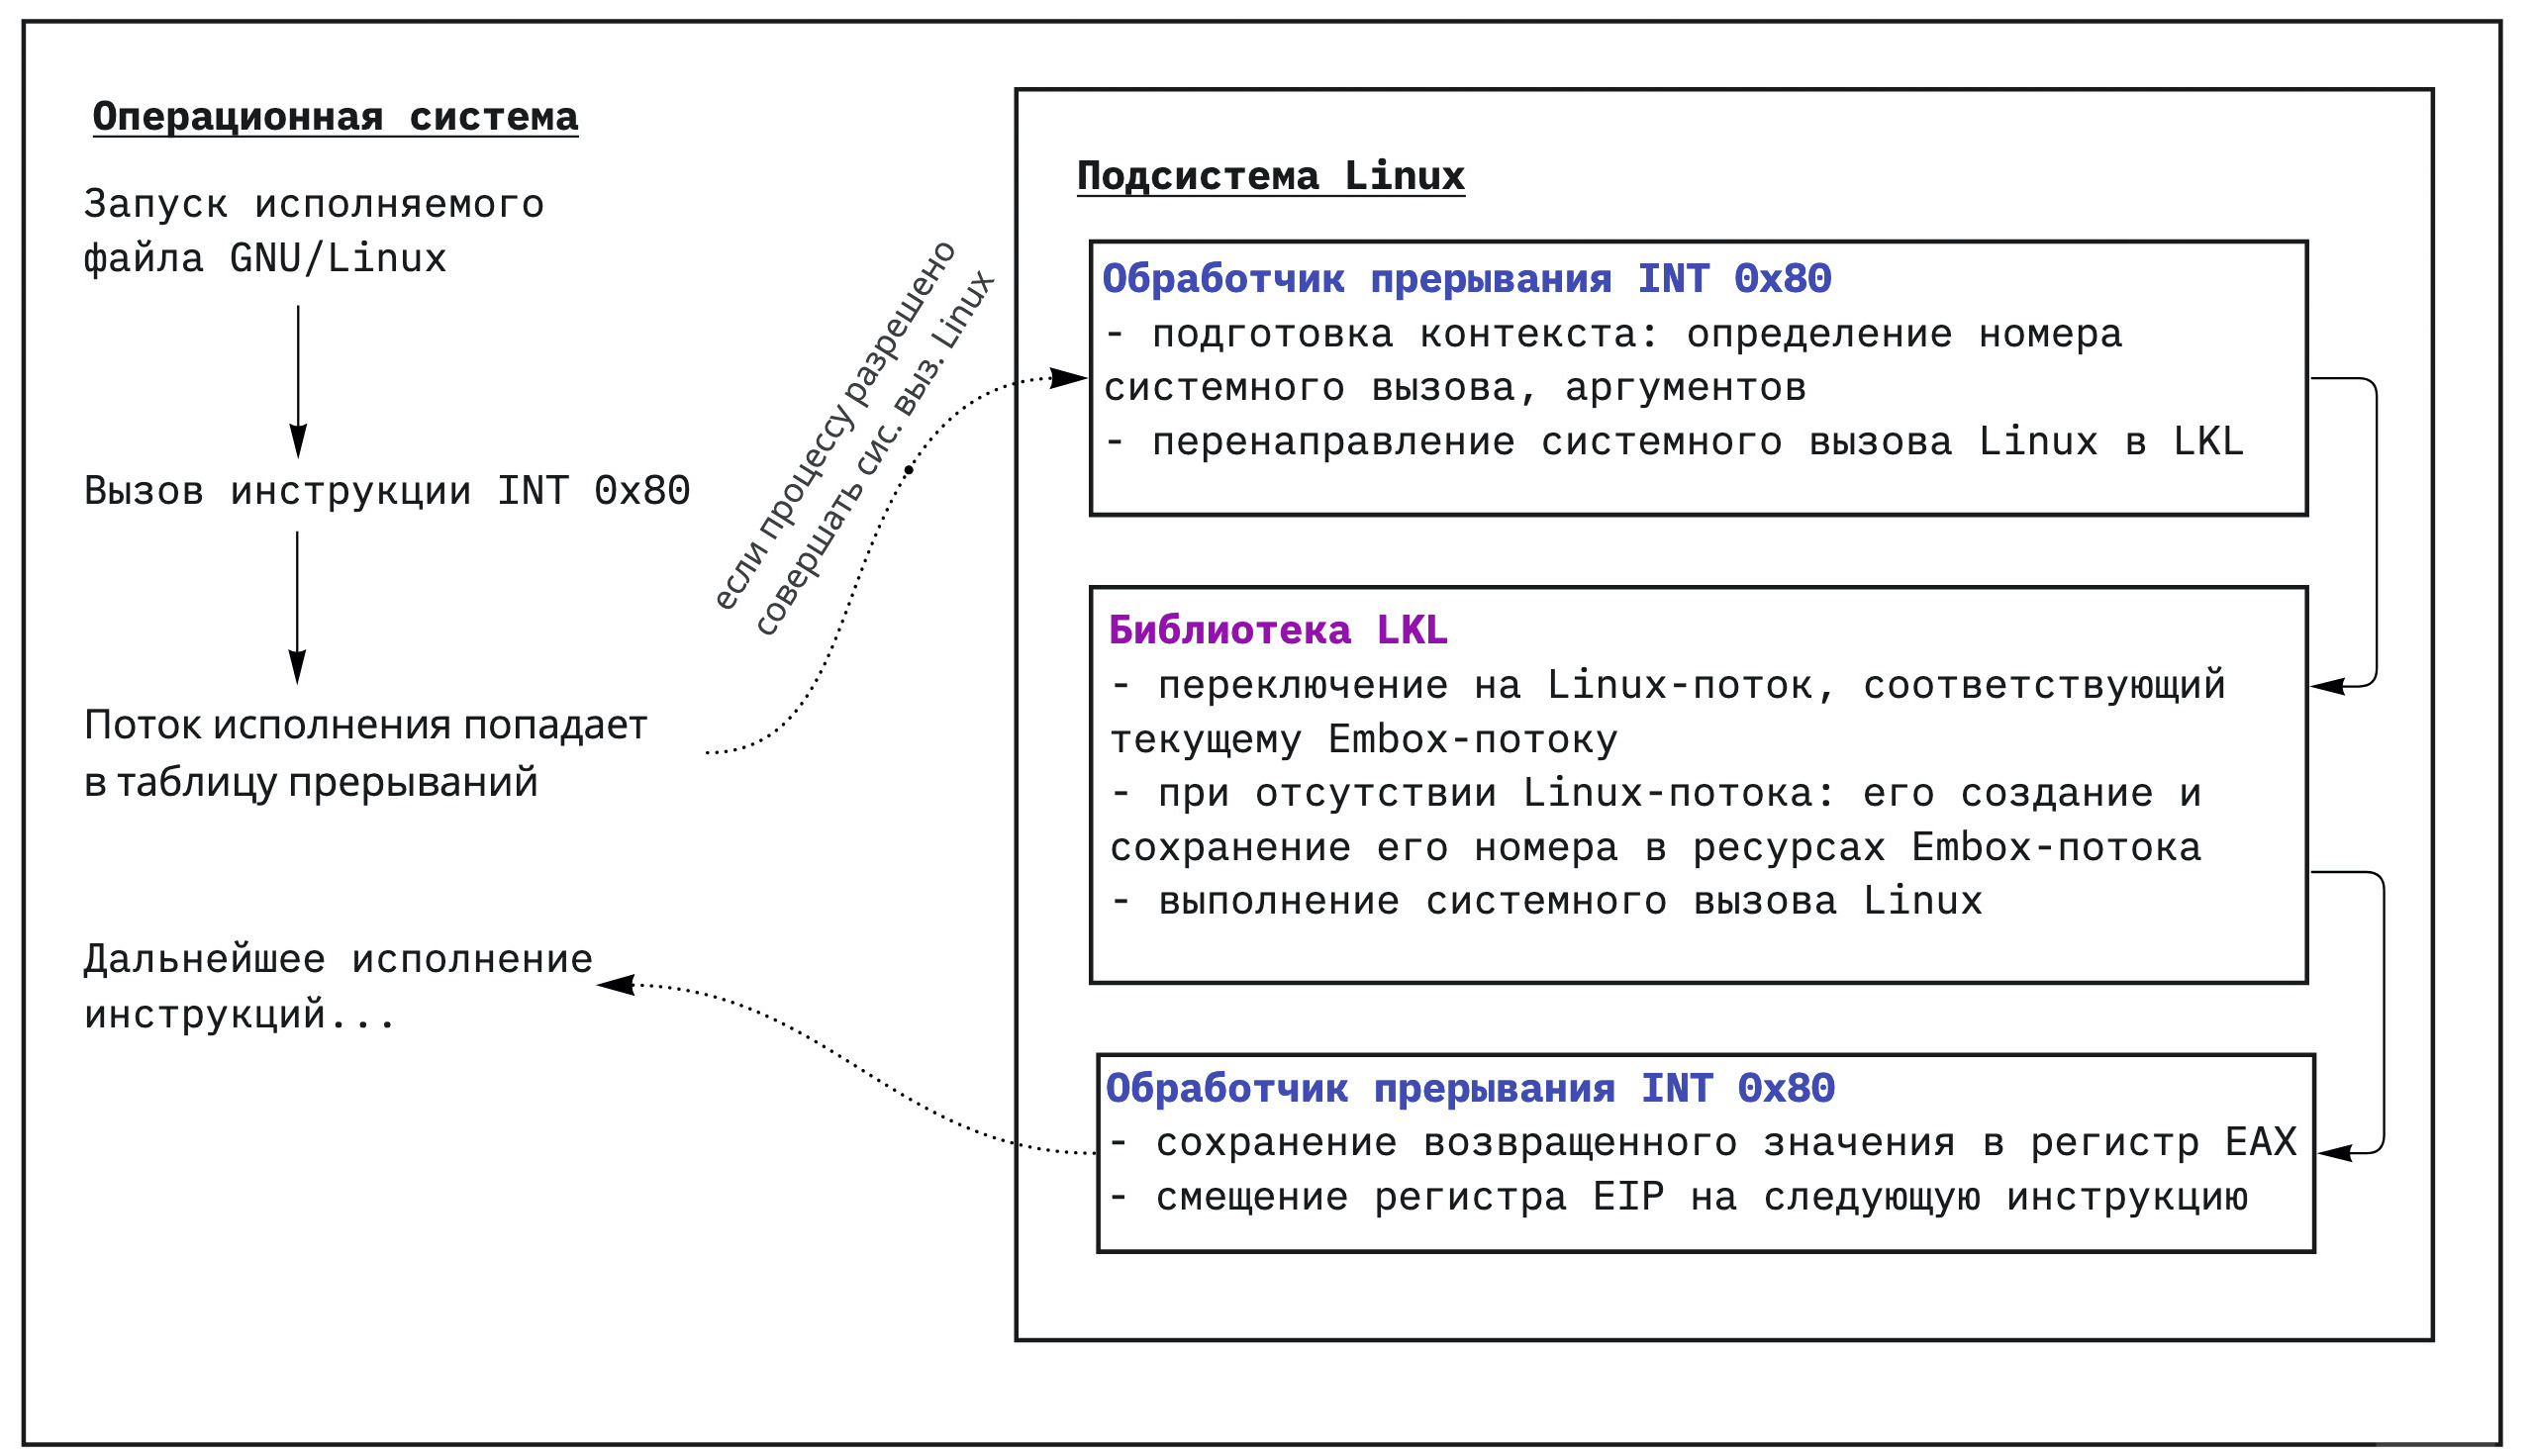
\includegraphics[width=\textwidth]{pictures/Arch.jpg}
\caption{Архитектура слоя совместимости}
\label{fig:arch}
\end{figure}


\section{Особенности реализации}
% !TeX spellcheck = ru_RU
% !TEX root = vkr.tex

На основе описанной архитектуры для ОС Embox был создан слой двоичной совместимости с приложениями GNU/Linux. Была реализована рассматриваемая в предыдущей главе подсистема, использующая в качестве паравиртуализируемого ядра Linux библиотеку LKL. Подсистема содержит все необходимые составляющие, включая функцию-обработчик системных вызовов Linux. К изменениям, затрагивающим концептуальные части исходного кода ОС Embox, можно отнести дополнение структуры задачи Embox полями для хранения ключа TLS и информации о разрешении на исполнение системных вызовов Linux. Автором был сформирован запрос на привнесение изменений в проект Embox~\cite{pull-request}.

Далее представлены некоторые детали реализации слоя двоичной совместимости с GNU/Linux, специфичные для ОС Embox. Описание некоторых их них может быть полезным при реализации слоя совместимости в других ОС.

% ----

\subsection{Модуль подсистемы Linux в ОС Embox}

В Embox все компоненты ОС существуют в виде модулей. Собираемый образ ОС будет содержать только те модули, которые были включены в файл конфигурации компонентов. Ранее библиотека LKL была внедрена в Embox в виде модуля~\cite{lkl-in-embox-patch}. Этот модуль был использован для реализации внутри ОС Embox упомянутой в разделе \ref{chapter-with-subsystem} подсистемы, осуществляющей инициализацию, настройку и проверку библиотеки LKL, а также реализующей функцию-обработчик системных вызовов Linux.

% ----

\subsection{Запуск сторонних исполняемых файлов}

Все программы и библиотеки в ОС Embox включаются в образ ОС на этапе сборки. Для запуска сторонних исполняемых файлов используется инструмент-загрузчик \texttt{load\_app}.

В структуру, отвечающую за представление задачи в ОС Embox, было добавлено поле для идентификации процесса как исполняющего двоичный код приложения Linux. Инструмент \texttt{load\_app} был модифицирован для идентификации процесса как исполняющего Linux приложение. Все дочерние процессы автоматически наследуют значение этого поля от родительского процесса при создании. Таким образом, пользователь разрешает исполнение системных вызовов Linux только тем процессам, которые создаются при вызове приложений Linux через инструмент \texttt{load\_app}.

% ----

\subsection{Вывод текста из LKL в терминал ОС Embox}

Часть взаимодействия между LKL и Embox происходит при помощи \textit{виртуальных блочных устройств} LKL. Благодаря этому механизму возможны такие действия, как вывод текста из LKL в терминал Embox, или взаимодействие Linux приложения с файловой системой Embox.

В подсистеме слоя совместимости было реализовано такое блочное устройство, которое выводит текст из LKL в терминал ОС Embox. Изначально LKL не имеет доступа к терминалу Embox. Для организации этого доступа в подсистеме с LKL создается \textit{виртуальное блочное устройство}, являющееся структурой \texttt{lkl\_disk}. Для этого блочного устройства определяются функции обработки запросов на чтение и запись. Далее, за блочным устройством закрепляется \textit{специальный блочный файл}, который имеет путь и имя \texttt{/vda}. Если системный вызов Linux \texttt{write} совершит запись в файловый дескриптор с номером 1 (стандартный вывод), то произойдёт запись информации в файл \texttt{/vda}. В \textit{обработчике запроса на запись} того устройства, на которое указывает файл \texttt{/vda}, реализован вывод текста в терминал ОС Embox (стандартными средствами Embox~--- функцией \texttt{printf}).

Подобных виртуальных устройств может быть произвольное количество, а обработчик каждого может обладать любым функционалом. Благодаря этому становится возможным, например, смонтировать в окружении подсистемы с ядром Linux файловую систему из ОС Embox для того, чтобы процесс мог работать с ней в контексте Linux.


\section{Тестирование и апробация}
% !TeX spellcheck = ru_RU
% !TEX root = vkr.tex

В среде ОС Embox были запущены некоторые приложения, осуществляющие системные вызовы Linux и скомпилированные для исполнения в среде ОС GNU/Linux.

Стоит отметить, что на момент написания данной работы в ОС Embox отсутствует возможность использовать механизм \textit{разделяемых библиотек} (англ. shared libraries). Это означает, что участвующие в апробации двоичные файлы должны быть скомпонованы полностью статически (не использовать механизм разделяемых библиотек). Даже простые программные инструменты в ОС GNU/Linux, такие как \texttt{echo}, напротив, компонуются динамически относительно библиотеки GLIBC\,\footnote{Например, даже такие функции как \texttt{write} и \texttt{read}, которые выглядят как <<прямые>> системные вызовы Linux, на самом деле являются функциями-обёртками, предоставляемыми библиотекой GLIBC.}. Более того, на практике очень сложно скомпоновать полностью статическую программу, если она использует GLIBC~--- библиотека не проектировалась для этого, попытки статической компоновки приведут к целому ряду проблем~\cite{glibc}. В качестве обходного пути можно попробовать использовать вместо GLIBC более подходящую для статической компоновки библиотеку, например библиотеку uClibc~\cite{uclibc}. Однако, автором был выбран иной путь~--- для ряда стандартных программных инструментов GNU/Linux были реализованы упрощённые аналоги, не использующие стандартную библиотеку Си. Для осуществления системного вызова Linux в этих программах используется аналог предоставляемой библиотекой GLIBC функции \texttt{syscall} (вызывает инструкцию \texttt{INT0x80} с заданными номером и аргументами системного вызова), на основе которого реализованы другие стандартные функции.

В первую очередь работоспособность модуля слоя двоичной совместимости была протестирована при помощи программы \texttt{linux\_echo}, выводящей передаваемый ей параметр в стандартный поток вывода (терминал). После компиляции программа работает как в среде GNU/Linux (рис.\,\ref{fig:linux_echo}), так и в среде ОС Embox (рис.\,\ref{fig:embox_echo}).

\begin{figure}[H]
\center{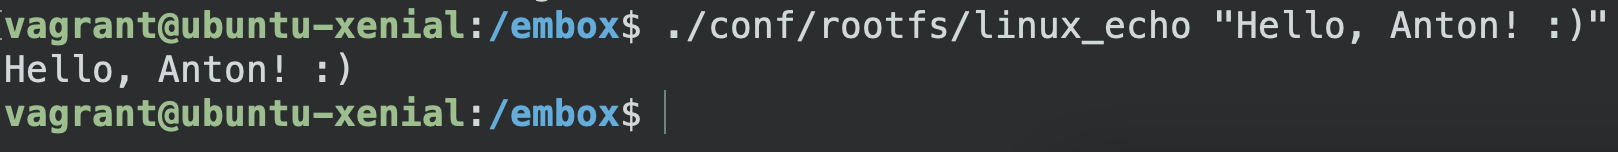
\includegraphics[scale=0.55]{pictures/linux_echo.png}}
\caption{Исполнение \texttt{linux\_echo} в ОС Ubuntu}
\label{fig:linux_echo}
\end{figure}

\begin{figure}[H]
\center{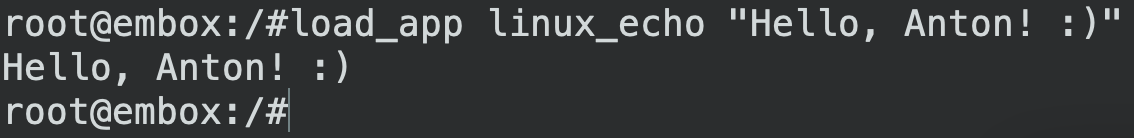
\includegraphics[scale=0.65]{pictures/embox_echo.png}}
\caption{Исполнение \texttt{linux\_echo} в ОС Embox}
\label{fig:embox_echo}
\end{figure}

Также, была продемонстрирована работа с \texttt{procfs}~--- специальной файловой системой Linux, предназначенной для получения некоторой служебной информации от ядра Linux. Эта файловая система реализуется в коде ядра Linux. Она не специфицирована, поэтому в ОС Embox может либо отсутствовать, либо иметь произвольную реализацию. Данный пример показывает, что программы GNU/Linux, которые зависят от подобных элементов ядра Linux, могут работать без необходимости реализации этих элементов в ОС Embox в том виде, в каком они существуют в ядре Linux (один из плюсов метода паравиртуализации).

Сначала в средах GNU/Linux (рис.\,\ref{fig:linux_ls}) и ОС Embox (рис.\,\ref{fig:embox_ls_root}, рис.\,\ref{fig:embox_ls_proc}) была запущена программа \texttt{linux\_ls}, выводящая содержимое заданного каталога. Затем, при помощи программы \texttt{linux\_cat} в обеих средах были прочитаны данные из некоторых файлов, предоставляемых файловой системой \texttt{procfs} (рис.\,\ref{fig:linux_cat}, рис.\,\ref{fig:embox_cat_devices}, рис.\,\ref{fig:embox_cat_stat}, рис.\,\ref{fig:embox_cat_slabinfo}).

\begin{figure}[H]
\center{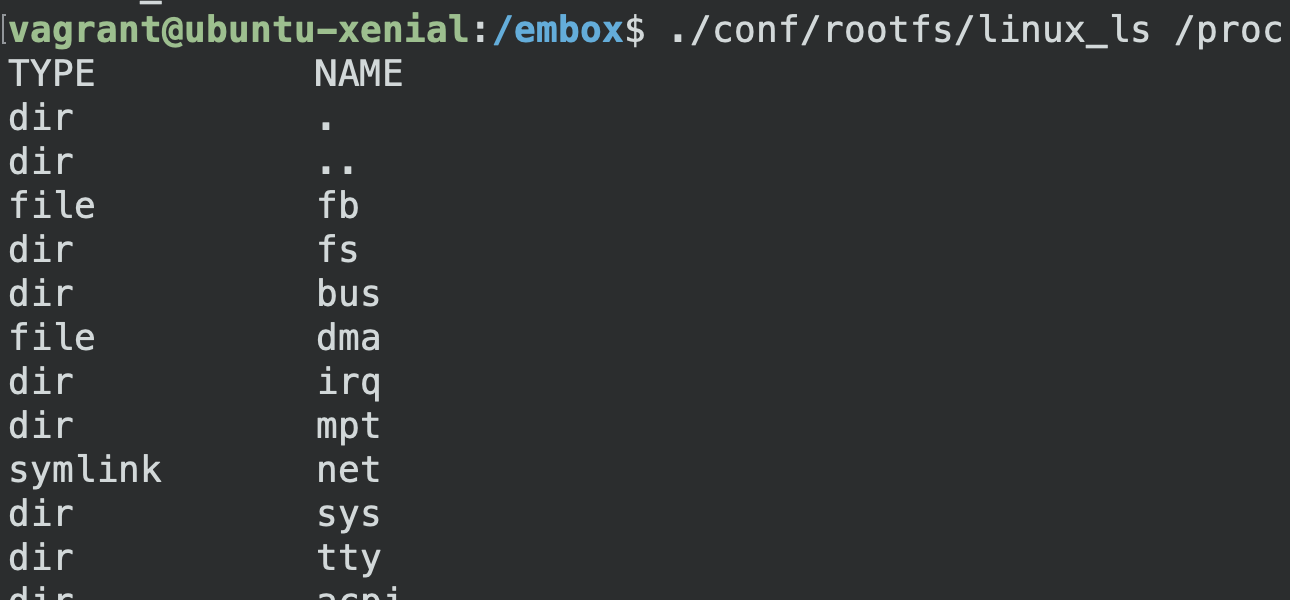
\includegraphics[scale=0.45]{pictures/linux_ls.png}}
\caption{Исполнение \texttt{linux\_ls} (каталог \texttt{/proc}) в ОС Ubuntu}
\label{fig:linux_ls}
\end{figure}

\begin{figure}[H]
\center{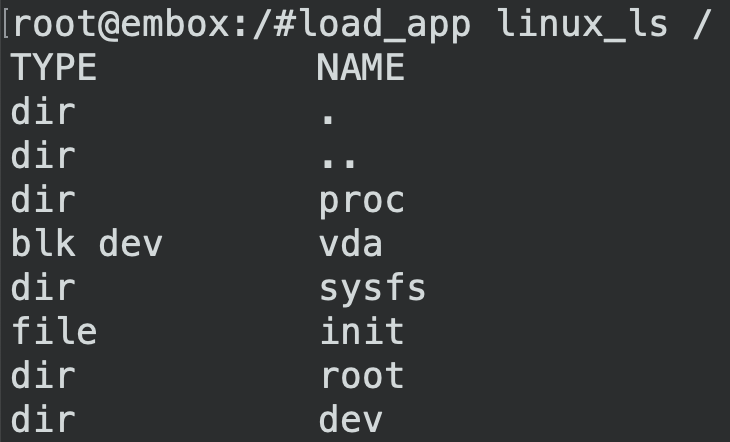
\includegraphics[scale=0.45]{pictures/embox_ls_root.png}}
\caption{Исполнение \texttt{linux\_ls} (корневой каталог) в ОС Embox}
\label{fig:embox_ls_root}
\end{figure}

\begin{figure}[H]
\center{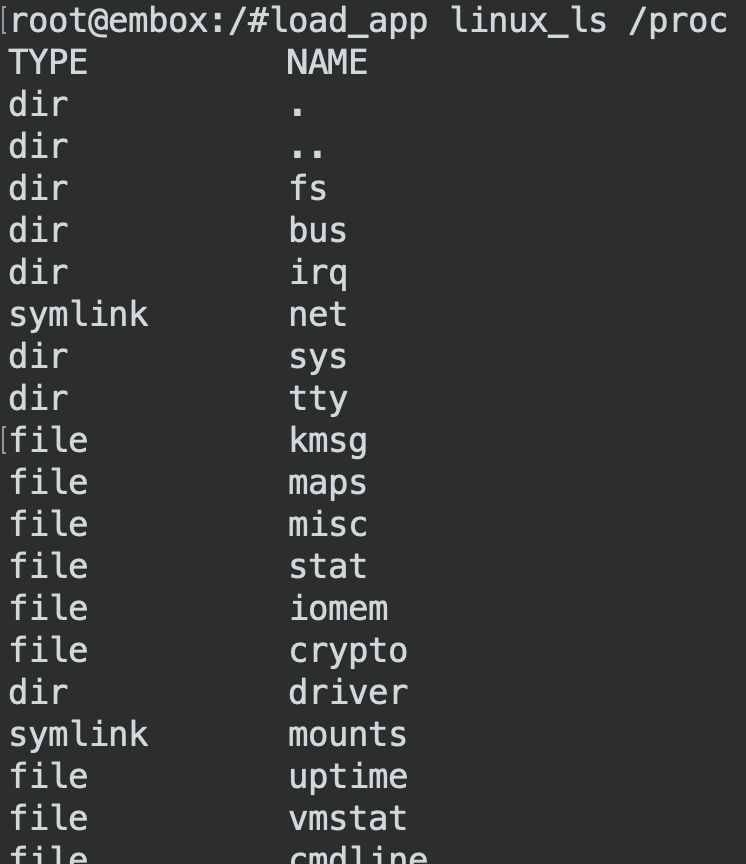
\includegraphics[scale=0.35]{pictures/embox_ls_proc.png}}
\caption{Исполнение \texttt{linux\_ls} (каталог \texttt{/proc}) в ОС Embox}
\label{fig:embox_ls_proc}
\end{figure}

\begin{figure}[H]
\center{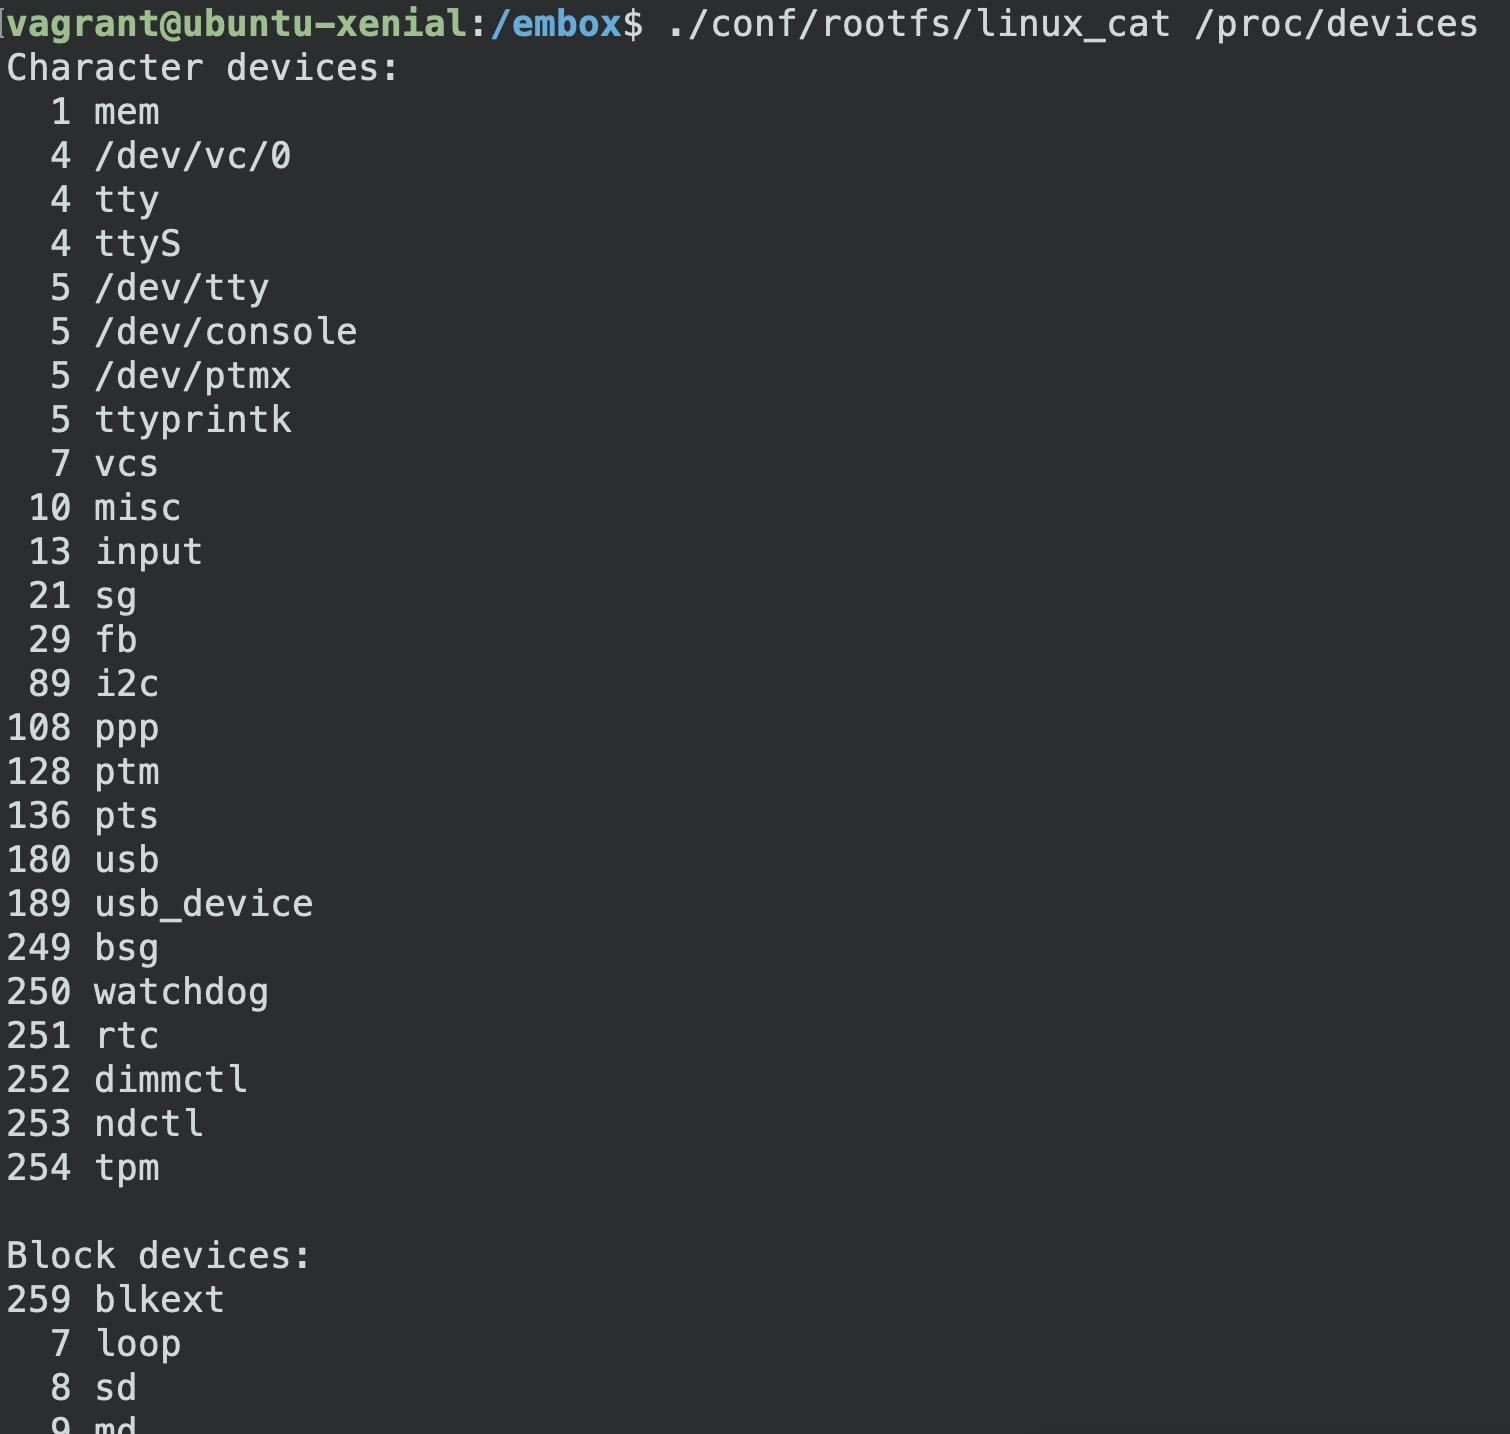
\includegraphics[scale=0.25]{pictures/linux_cat.png}}
\caption{Исполнение \texttt{linux\_cat} (файл \texttt{/proc/devices}) в ОС Ubuntu}
\label{fig:linux_cat}
\end{figure}

\begin{figure}[H]
\center{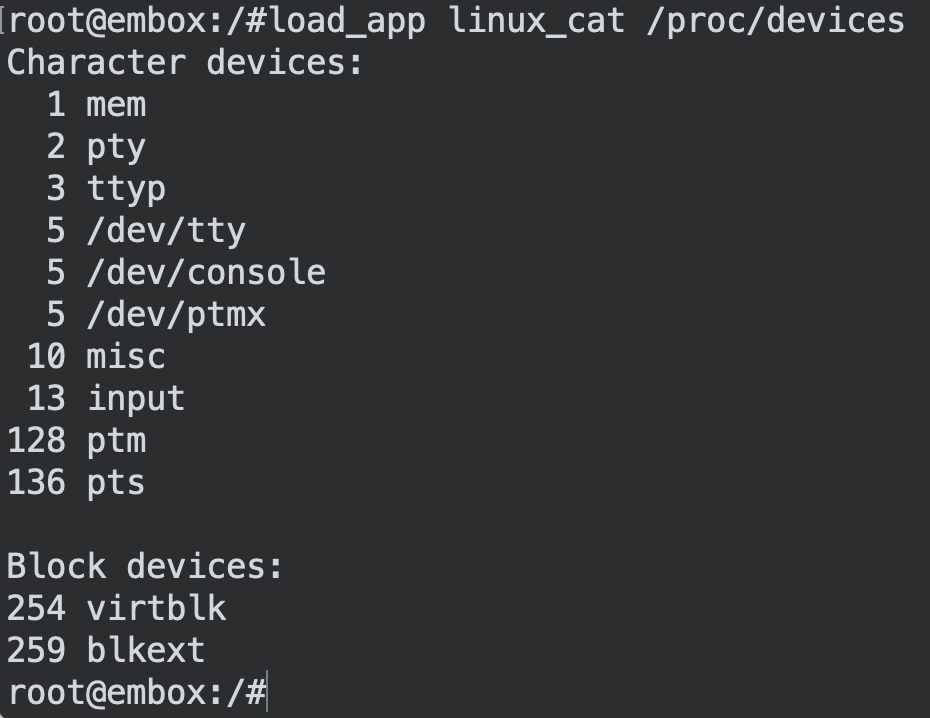
\includegraphics[scale=0.45]{pictures/embox_cat_devices.png}}
\caption{Исполнение \texttt{linux\_cat} (файл \texttt{/proc/devices}) в ОС Embox}
\label{fig:embox_cat_devices}
\end{figure}

\begin{figure}[H]
\center{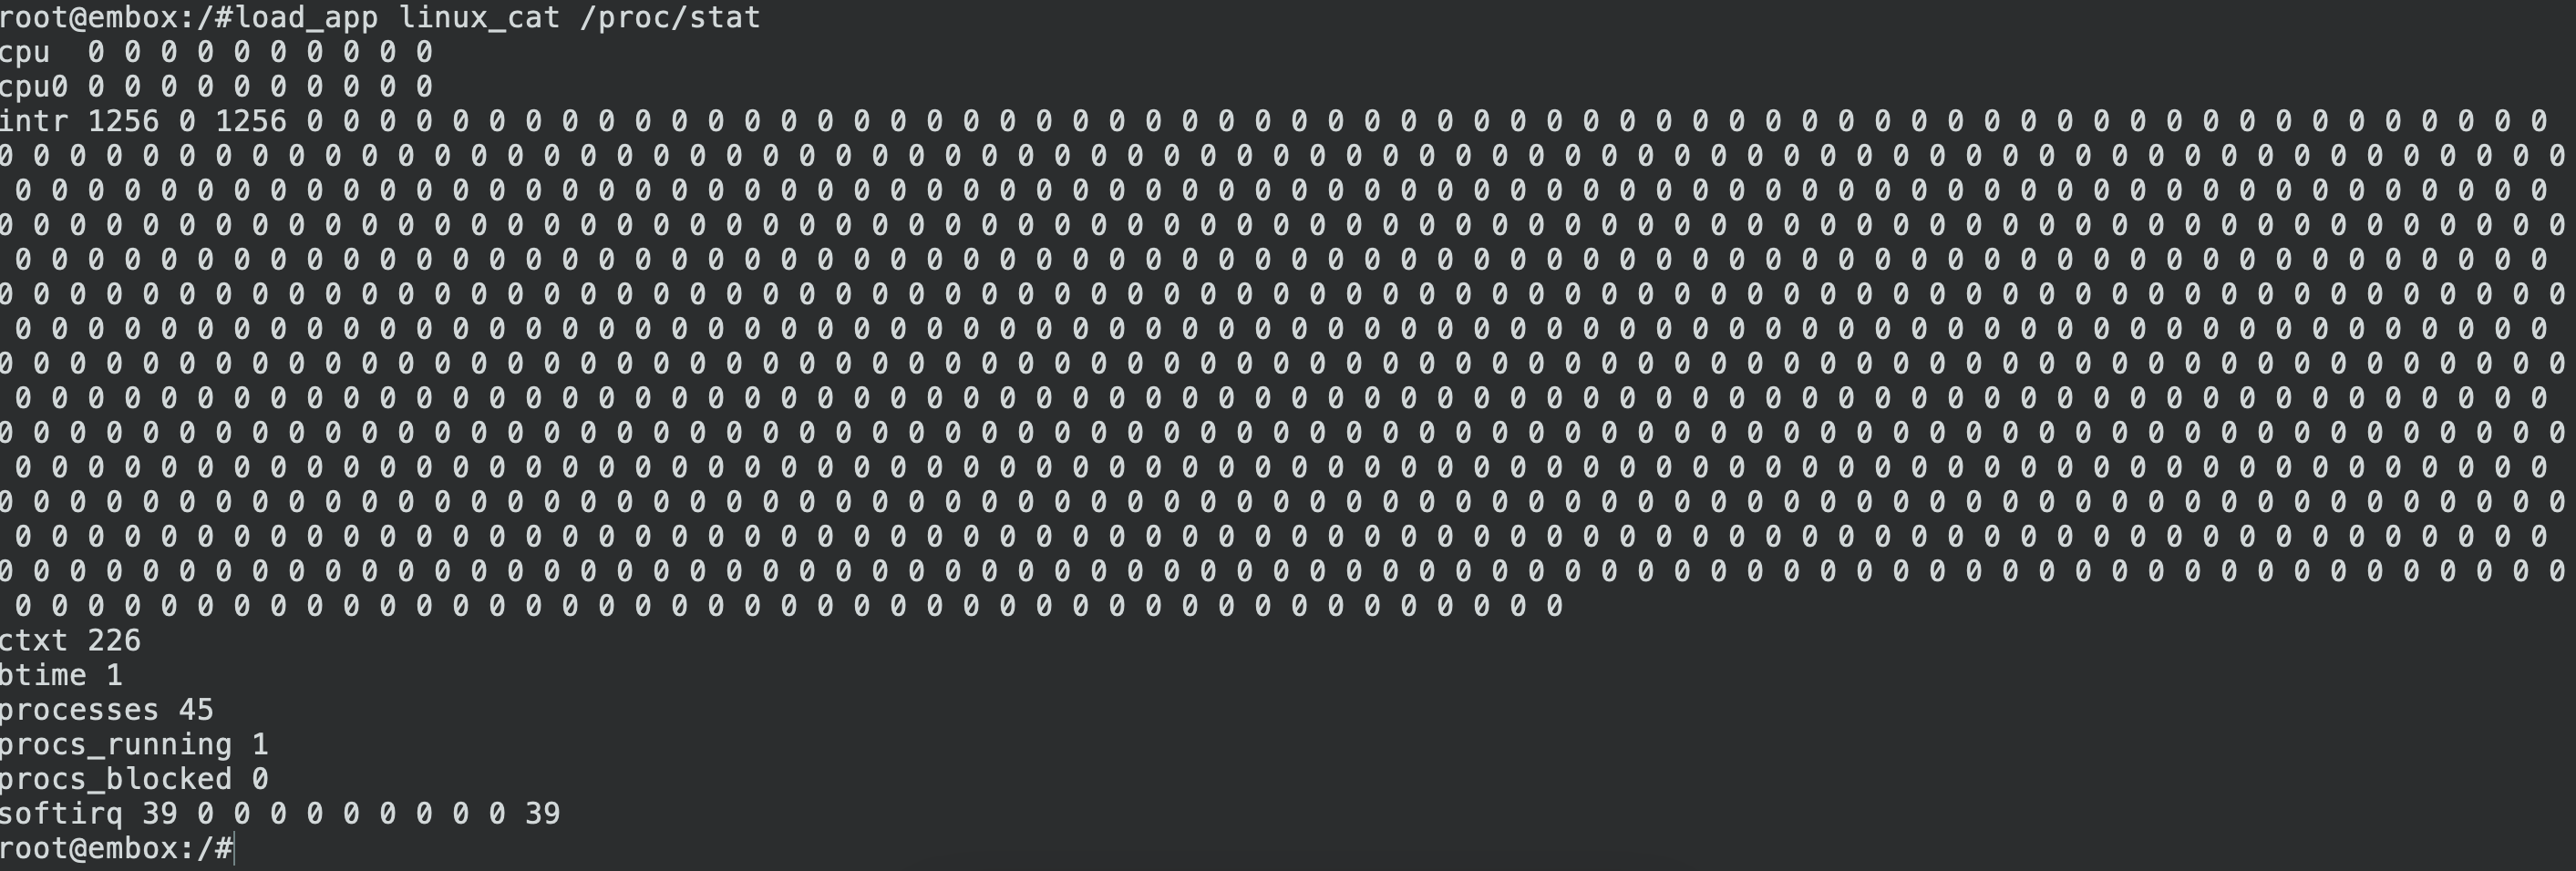
\includegraphics[scale=0.25]{pictures/embox_cat_stat.png}}
\caption{Исполнение \texttt{linux\_cat} (файл \texttt{/proc/stat}) в ОС Embox}
\label{fig:embox_cat_stat}
\end{figure}

\begin{figure}[H]
\center{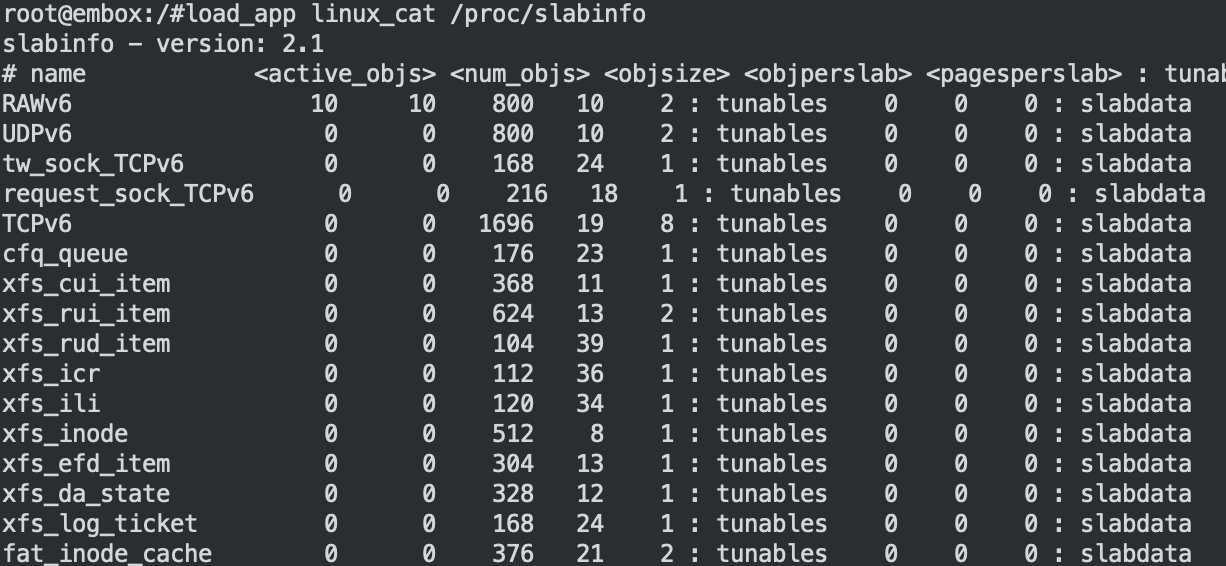
\includegraphics[scale=0.45]{pictures/embox_cat_slabinfo.png}}
\caption{Исполнение \texttt{linux\_cat} (файл \texttt{/proc/slabinfo}) в среде Embox}
\label{fig:embox_cat_slabinfo}
\end{figure}

Такая демонстрация задействует всю цепочку компонентов слоя двоичной совместимости. В ОС Embox есть два разных окружения~--- одно является обычным окружением Embox, другое предоставляется реализованной подсистемой. В среде Embox запускаются приложения, совершающие системные вызовы Linux. Паравиртуализируемое ядро Linux (библиотека LKL) выполняет обработку этих системных вызовов. Виртуальное устройство внутри LKL успешно выводит текст на терминал Embox. Процессу ОС Embox доступно как обычное окружение Embox, так и окружение, предоставляемое подсистемой с ядром Linux.


\section*{Заключение}
% !TeX spellcheck = ru_RU
% !TEX root = vkr.tex

В рамках данной работы были достигнуты следующие результаты.
\begin{itemize}
  \item Проведён анализ существующих в разных ОС реализаций слоя двоичной совместимости с GNU/Linux. Выделены два подхода: эмуляция и паравиртуализация. Сделан выбор в пользу метода паравиртуализации ядра Linux.
  \item Разработана архитектура подсистемы двоичной совместимости с GNU/Linux, которая может быть реализована в ряде разных ОС. Это достигается за счёт использования библиотеки LKL в качестве паравиртуализированного ядра.
  \item На основе разработанной архитектуры реализована и настроена подсистема для ОС Embox.
  \item Проведена апробация созданной подсистемы. В Embox запущены демонстрационные приложения \texttt{linux\_cat} и \texttt{linux\_ls}. Продемонстрирована работа с файловой системой \texttt{procfs}.
\end{itemize}

Логичным продолжением данной работы будет являться исследование возможности поддержки слоем совместимости разделяемых библиотек и запуска двоичных файлов, скомпонованных динамически. В частности, поддержка библиотеки GLIBC (как разделяемой) сильно увеличит область применимости предлагаемого слоя двоичной совместимости.


\setmonofont[Mapping=tex-text]{CMU Typewriter Text}
  \bibliographystyle{ugost2008ls}
  \bibliography{vkr}
\end{document}
